\capitulo{3}{Conceptos teóricos}

En este apartado se explican conceptos los básicos necesarios para entender el contexto en que se desarrolla este proyecto, respecto a lo que aquí se pretende, haciendo hincapié en la topografía y el dibujo en CAD. 

\section{Levantamiento topográfico}

Un levantamiento topográfico consiste en la medición de distintos puntos, mediante cálculos topográficos, donde se obtienen las coordenadas de estos, generalmente las coordenadas $X$, $Y$ y $Z$. Estas coordenadas nos indican su posición exacta en el espacio. 

El software que tienen los equipos de topografía; como teodolitos, estaciones totales o GPS, permiten asociar a cada punto un texto en el momento de medir el punto y así, el punto queda registrado con ese campo.

Este campo de texto, que de aquí en adelante llamaremos código de punto, es el elemento en el que se centra este proyecto. El algoritmo diseñado debe saber interpretar este código de punto. Como veremos más adelante, este nos puede indicar una o múltiples cosas a la vez, lo que conlleva mayor dificultad a la hora de definir el formato que debe tener este. Tiene que aportar la máxima información posible, pero a la vez tiene que ser muy sencillo en su estructura y de una longitud lo más corta posible. No es muy viable tener que estar mucho tiempo tecleando, ya que se perdería mucho tiempo y alargaría en exceso el trabajo de campo.

\section{Archivo DXF---Elementos del dibujo}

DXF (acrónimo del inglés \emph{Drawing Exchange Format}) es un formato de archivo para dibujos de diseño asistido por computadora, creado por \emph{AutoCAD}. Formato muy extendido y utilizado por la mayoría de programas de CAD, como por ejemplo: \emph{AutoCAD, MicroStation, FreeCAD, DraftSight},... y también por programas de GIS, como: \emph{ArcGIS, QGIS, gvSIG}, ...

Para entender de forma sencilla los elementos de los que está compuesto un archivo DXF, solo se tratarán aquellos elementos que se utilizan en esta aplicación, de otra forma, la explicación sería muy extensa.
Simplificando, se procede a hacer una diferenciación entre los elementos que queremos dibujar, que llamaremos elementos gráficos, y los elementos no gráficos.

\textbf {Elementos gráficos}
\begin{itemize}
\item\textbf{Puntos:} En este caso es el elemento básico, ya que en una medición topográfica solo se obtienen puntos. El resto de los elementos que se exponen a continuación están basados en la posición de estos puntos.

\item\textbf{Líneas:} Están formadas por una sucesión de puntos, pueden ser abiertas o cerradas. Deben tener un punto inicial y otro final. Los cuadrados y rectángulos, en esta aplicación, se pueden englobar en este grupo, al ser polígonos o líneas cerradas.

\item\textbf{\emph{Splines}:} Curvas interpoladas en una sucesión de puntos, pueden ser abiertas o cerradas. Deben tener un punto inicial y otro final.

\item\textbf{Círculos:} En esta aplicación los definiremos por un punto, que es el centro del círculo y un radio.

\item\textbf{Textos:} Es un texto cuya posición en el dibujo se define, por la posición de un punto y una distancia a este.

\end{itemize}


\begin{figure}[!h]
	\centering
	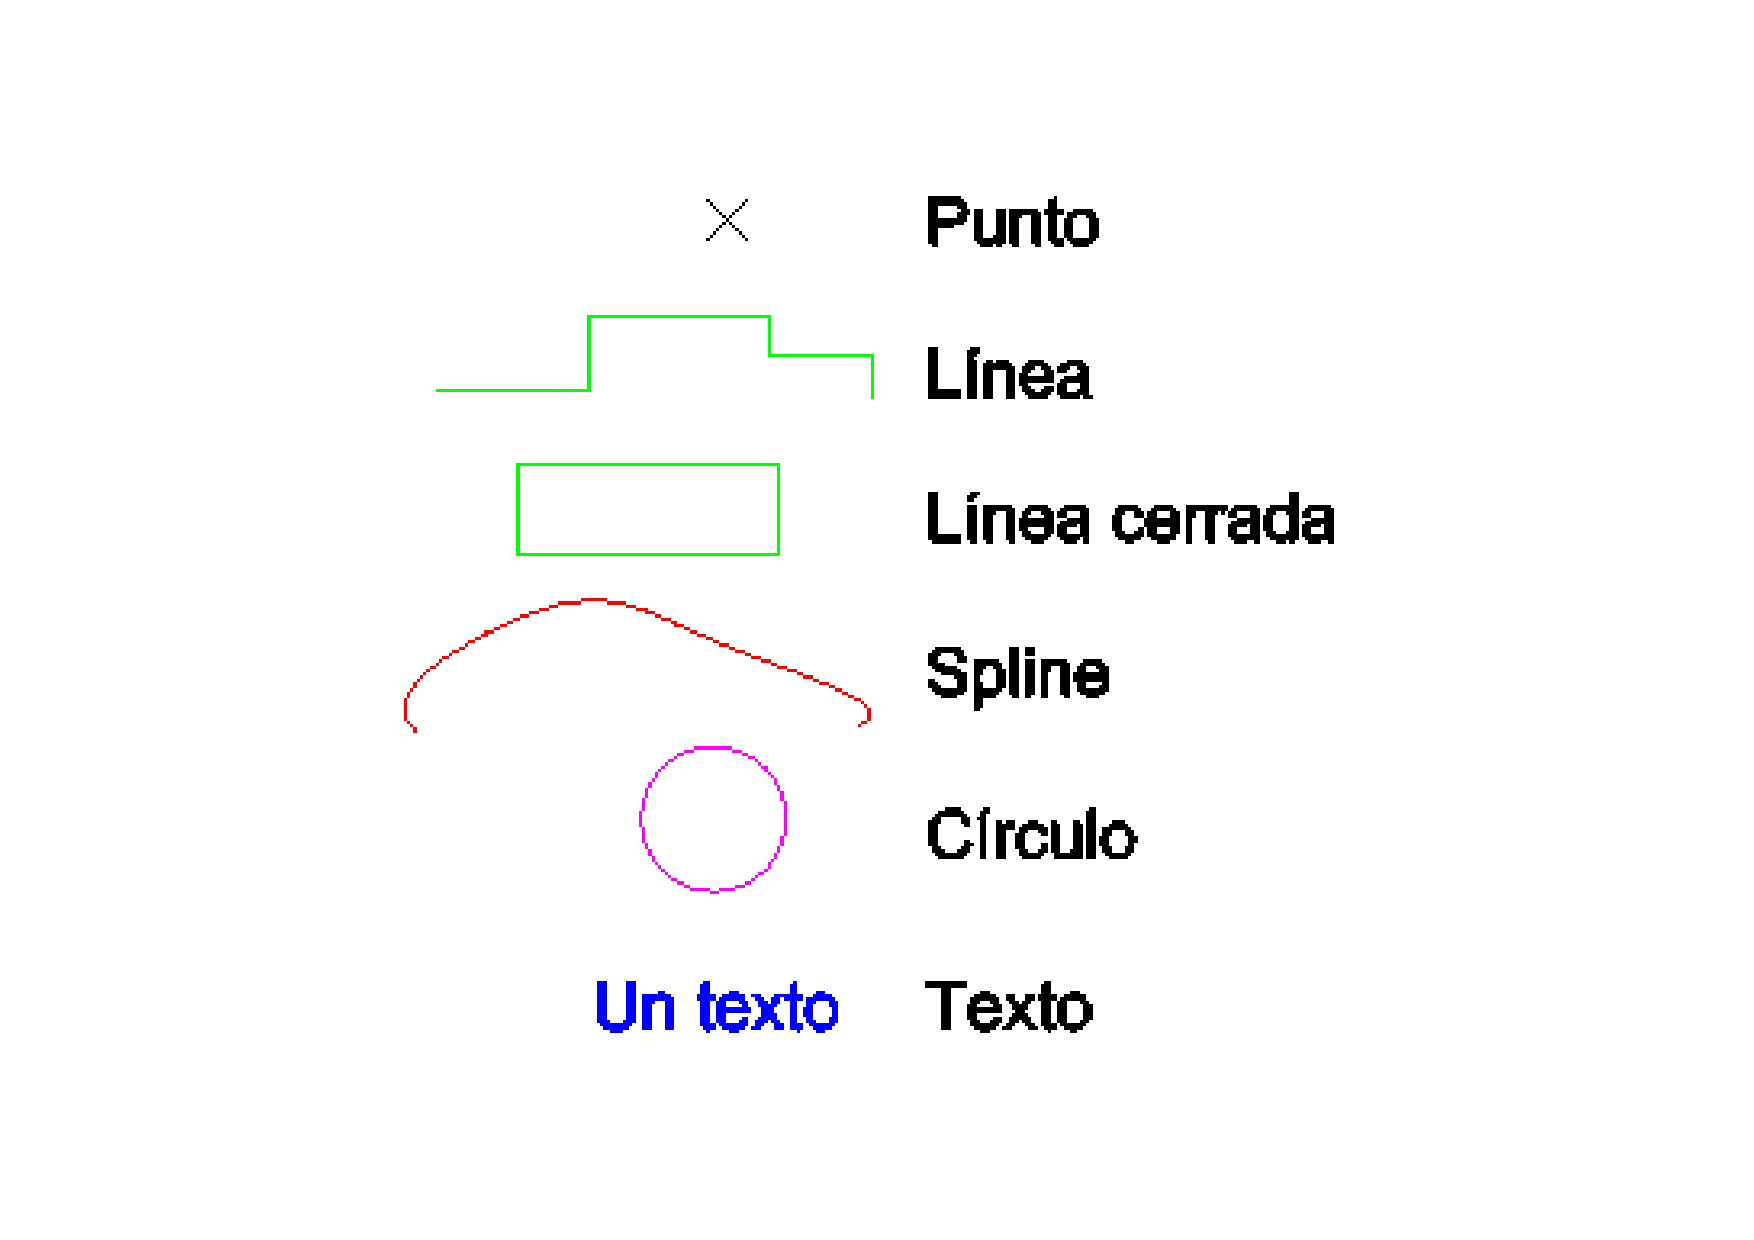
\includegraphics[width=0.5\textwidth]{Tipos}
	\caption{Elementos gráficos.}
	\label{fig:Tipos}
\end{figure}

\newpage

\textbf {Elementos no gráficos}

\begin{itemize}

\item\textbf{Capas:} Sirven para organizar mejor los objetos en nuestro dibujo ayudando a un mejor manejo a la hora de mover, copiar o identificarlos en el plano. Estas son un aspecto fundamental en el desarrollo del dibujo para poder obtener un plano bien organizado y con excelente presentación. En un buen trabajo, es casi imprescindible el uso de capas.

Las capas son una forma de clasificar objetos en CAD, si tienes un plano muy extenso con muchos objetos, la forma más fácil de identificarlos es mediante su capa, cada objeto dibujado en CAD se le asociara una capa y esa capa la puedes crear asignándole un nombre y un color, entre otras cosas. Es la mejor forma de identificar cierto objeto dentro de tu dibujo.
En esta aplicación, las capas tendrán un nombre y un color.

\imagen{capas}{Capas en un programa de CAD}

\item\textbf{Bloques:} Un bloque en CAD es un conjunto de objetos (llamados entidades), agrupados como un todo. Es decir, que podemos dibujar líneas, arcos, círculos, cada uno con propiedades distintas que los demás y luego invocar un comando para <<juntarlos>> a todos bajo un mismo nombre y asignarle un punto de inserción.

En esta aplicación se pretende que el usuario pueda subir un archivo DXF personalizado con sus bloques, y poder asignarlo a diferentes puntos del levantamiento topográfico a través del código de punto


\begin{figure}[!h]
	\centering
	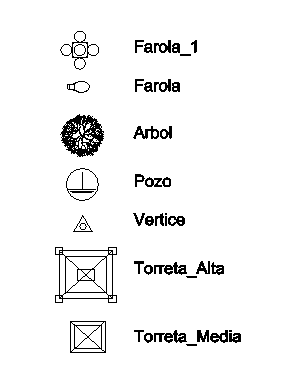
\includegraphics[width=0.4\textwidth]{Simbolos}
	\caption{Símbolos creados como entidades bloques de CAD.}
	\label{fig:Simbolos}
\end{figure}

\end{itemize}

\section{Codificación de los puntos}\label{sec:codificacion}

Como se ha mencionado anteriormente, la codificación de los puntos es la parte clave para el desarrollo de este proyecto, ya que en ella se va a basar la aplicación a la hora de crear los elementos del dibujo.
Debe poder crear líneas y \emph{splines}, interpretando donde empiezan y acaban. Crear círculos, cuadrados y rectángulos, insertar símbolos o bloques en determinados puntos y, por último, asociar cada elemento su capa correspondiente, con su color asignado.

Todo esto, si eres un usuario con conocimientos en manejo de aplicaciones CAD, se haría de forma manual en su mayor parte. Con una buena definición del código de punto, se tratará de automatizar todo este proceso.
Como ya sabemos, el código debe ser lo mas sencillo posible y a la vez aportar la máxima información posible, dejando que el usuario tenga libertad para elegir los códigos, salvo algunas partes, que deben de tener una sintaxis concreta. 

A continuación, veremos algunos ejemplos de codificación para distintos elementos del dibujo:

\begin{itemize}

\item Se quiere dibujar la línea que define el arcén de una carretera, podríamos escribir en el código del punto; ‘ARCEN’, ‘ARC’, ‘A’, o lo que quisiéramos. Como se pretende que el código sea lo más sencillo posible, tomamos como mejor opción ‘A’. Para definir que la línea empieza en un punto concreto, ese texto debe ir seguido obligatoriamente del carácter ‘I’. Un ejemplo de cómo sería una línea de arcén formada por 4 puntos es: (‘A I’, ‘A’, ‘A’, ‘A’).


\begin{figure}[!h]
	\centering
	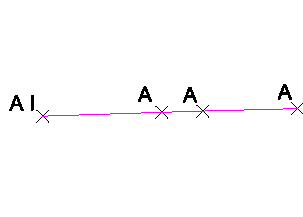
\includegraphics[width=0.6\textwidth]{Polilinea}
	\caption{Representación de una línea.}
	\label{fig:Polilinea}
\end{figure}

\item Siguiendo con el ejemplo anterior, ahora queremos que dibuje una curva tipo \emph{spline}. Para definir que la línea empieza en un punto concreto y que sea \emph{spline}, ese texto debe ir seguido obligatoriamente del carácter ‘IC’ y el resto de los puntos de esa curva, el texto inicial debe ir seguido obligatoriamente del carácter ‘C’. Un ejemplo de cómo sería una línea de arcén tipo \emph{spline} formada por 4 puntos es: (‘A IC’, ‘AC’, ‘AC’, ‘AC’).

\begin{figure}[!h]
	\centering
	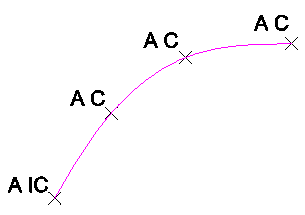
\includegraphics[width=0.6\textwidth]{Splines}
	\caption{Representación de una curva \emph{Spline}.}
	\label{fig:Splines}
\end{figure}

\item Se quiere dibujar un cuadrado, por ejemplo, una tapa de registro perteneciente a la red de saneamiento. El código de punto debe comenzar obligatoriamente por ‘TC’, seguido de la descripción que queramos asignarle, en este caso como es la red de saneamiento usaremos ‘SAN’. Así finalmente, el código para ese punto queda ‘TC SAN’. Como se pretende optimizar también el trabajo de campo, un cuadrado solo se definirá mediante 2 puntos y la aplicación al interpretar el código, deberá siempre dibujar un cuadrado a la derecha de esos dos puntos. La explicación es sencilla, si en un trabajo hay que medir 500 tapas de registro, no es lo mismo medir 1000 puntos que 2000. Con esta codificación nos hemos ahorrado la mitad del tiempo en el trabajo de campo.

\item Lo mismo que en el caso anterior, para dibujar rectángulos. El código de punto debe comenzar obligatoriamente por ‘TR’, seguido de la descripción que queramos asignarle, en este caso como es la red de saneamiento usaremos ‘SAN’. Así finalmente, el código para ese punto queda ‘TR SAN’. Como se pretende optimizar también el trabajo de campo, un rectángulo solo se definirá mediante 3 puntos y la aplicación al interpretar el código, deberá siempre dibujar un rectángulo.

\item Se quiere dibujar un círculo, por ejemplo, una tapa de registro perteneciente a la red eléctrica.  El código de punto debe comenzar obligatoriamente por ‘TX’, seguido de la descripción que queramos asignarle, en este caso como es la red de eléctrica usaremos ‘RE’. En este código necesitaremos también incluir en radio de la circunferencia, por ejemplo 0.5 metros, por lo que al final el código queda ‘TX 0.5 RE’.


\begin{figure}[!h]
	\centering
	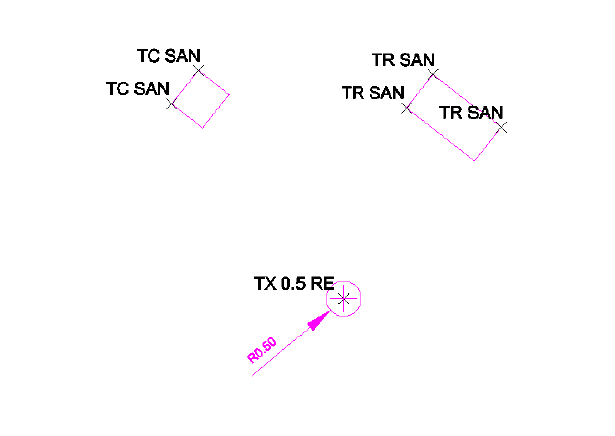
\includegraphics[width=0.8\textwidth]{CRC}
	\caption{Representación de un rectángulo, un cuadrado y un círculo.}
	\label{fig:CRC}
\end{figure}

\item Por último, planteamos una opción más complicada, que suele ser habitual en los trabajos de campo, la representación de elementos que realmente no se han medido en campo, porque pueden no ser accesibles. Queremos representar la línea de la fachada de un edificio, donde existen dos puntos inaccesibles, que no podemos medir topográficamente, pero conocemos su longitud (por ejemplo, hemos extraído estos datos de un plano catastral). Como es un edificio, podríamos representarlo con el texto ‘E’. La siguiente secuencia de 4 puntos con su codificación, construirá la línea final formada por 6 puntos, (‘E I’,’E 1.5 -2’,’E’,’E’). El código el punto 2, ’E 1.5 -2’, indica que cuando la línea llegue a ese punto, debe continuar perpendicular a su derecha durante 1.5 metros, después, 2 metros, también en perpendicular, hacia su izquierda, y por último debe unirse con el siguiente punto que forma la línea. 

\begin{figure}[!h]
	\centering
	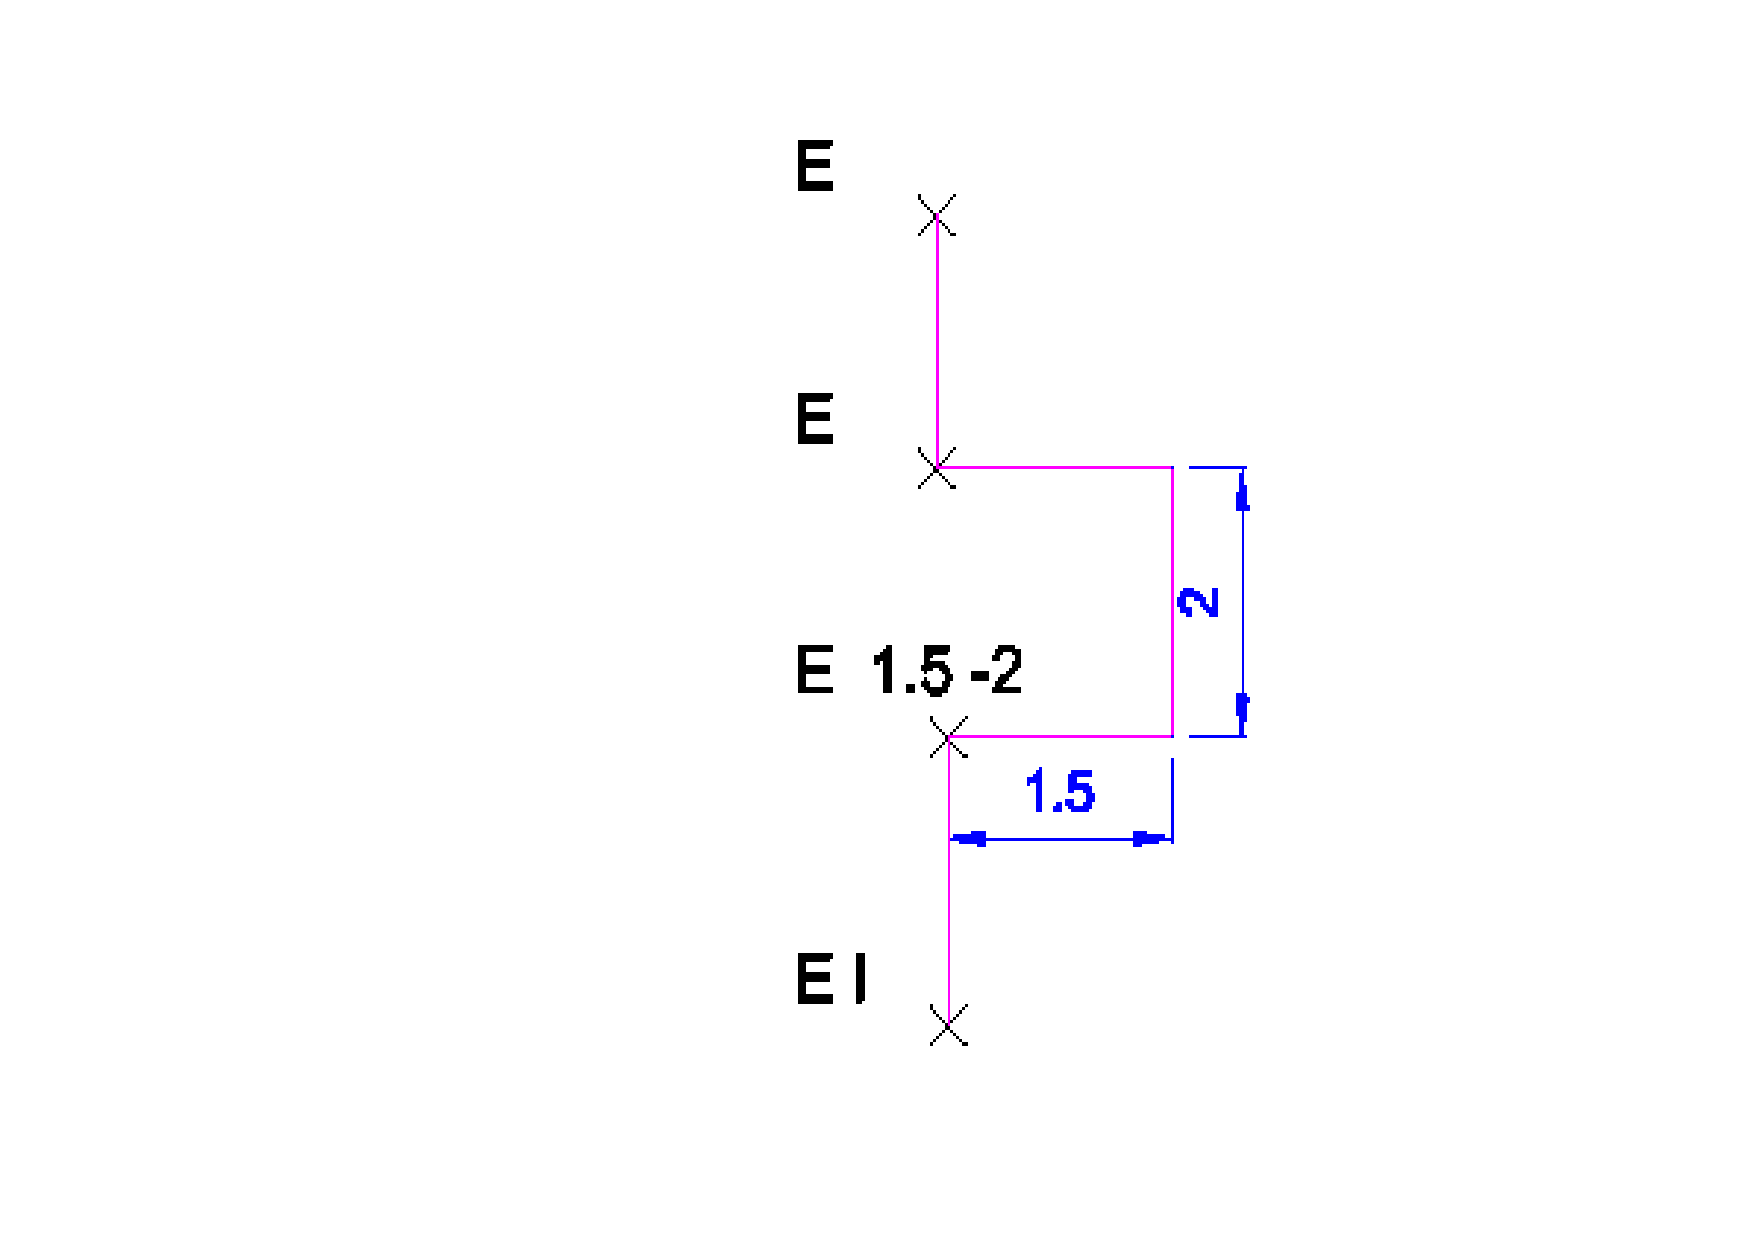
\includegraphics[width=0.6\textwidth]{Inaccesibles}
	\caption{Representación de como se crearía una línea formada por puntos inaccesibles.}
	\label{fig:Inaccesibles}
\end{figure}


\end{itemize}

Otra gran ventaja que aporta esta codificación es que los puntos en campo que forman un elemento no estás obligado a medirlos de forma consecutiva, lo que supone un importantísimo ahorro de tiempo. Vamos a explicar esto con un ejemplo.

Se pretende dibujar el plano de una carretera de 50 km, las líneas que nos interesan son; el eje de la carretera y las líneas de los arcenes. No podemos plantearnos el medir las líneas de forma consecutiva, por ejemplo, medir el arcén derecho, volver por el eje y, por último, el arcén izquierdo. Si hiciéramos esto, recorreríamos 150 km. Esta aplicación es capaz de crear distintas líneas, aunque no estén medidas en campo en un orden consecutivo. Una solución de codificación podría ser la siguiente secuencia de puntos: (‘AD I’,’E I’,’AI I’,’AI’,’E’,’AD’,’E’,’AD’,’AI’,…), donde ‘AD’ es el arcén derecho, ‘E’ el eje, ‘AI’ el arcén izquierdo. Así solo recorreríamos la carretera una sola vez. 

Vemos que este tipo de codificación definida no solo aporta la ventaja de generar automáticamente el plano, si no que, el tiempo ahorrado en el trabajo de campo, es la mayor ventaja. Esta parte del trabajo es la que tiene mayores costes y, por lo tanto, más peso a la hora de decidirse por un proyecto.

\tablaSmall{Caracteres obligatorios y significado.}{l c 
}{codigos}
{ \multicolumn{1}{l}{Caracter} & Significado \\}{ 
'I'	& Punto inicio de línea\\
'IC'& Punto inicio de curva\\
'C' & Punto perteneciente a una curva\\
'TC'& Punto perteneciente a un cuadrado\\
'TR'& Punto perteneciente a un rectángulo\\
'TX'& Punto que define un círculo\\
}